\chapter{Tractor Simple}\label{chap:tractorsimple}
\section{Case Description}
The "Tractor Simple" demonstrates a model of a Lego\textregistered
Mindstorms\textregistered NXT tractor (micro-tractor), used to
demonstrate agricultural route planning and execution.  A pre-planned
route for the micro-tractor is supplied in advance (see figure
\ref{subfig:tractorSimple_a}).  The onboard system then aims to adjust
the current position so it gets as close as possible to the
pre-planned route.  The ability to automatically correct the position
helps deal with physical conditions, which may affect the vehicle's
movements in unpredictable ways.

\begin{figure}[!ht]
  \centering
 \subfigure[Micro-tractor with an example route-plan]{
  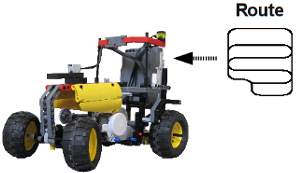
\includegraphics[height=3.6cm]{TractorSimple/tractorSimple_Overview.png}
  \label{subfig:tractorSimple_a}
  }
  \hspace{1cm}
  \subfigure[Sketch of the micro-tractors steering and drive components.]{
  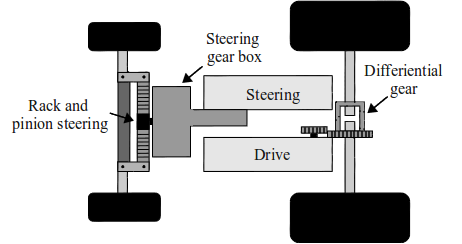
\includegraphics[height=3.6cm]{TractorSimple/tractor_sketch.png}
  \label{subfig:tractorSimple_b}
  }
\end{figure}

Two DC-motors on the micro-tractor are used to steer the front-wheels
and drive the back-wheels (see figure \ref{subfig:tractorSimple_b}).
%A localized reference system based on the motor-encoders and IMU (Iertial Measurement Unit) values is used to determine the current position.
The current route segment (straight line, turn/circle) in the
pre-planned route is followed until the controller determines a new
segment must be loaded.  When the micro-tractor has fished the
pre-planned route, it stops and ends the execution phase.

\section{External Links}
The purpose of this model was to model the general behaviour of the
micro-tractor, when running a pre-planned route and compared
successfully against the real system in \cite{Christiansen&12a}.
Using the \DESTECS model for tuning optimized control parameters for
the route-following algorithm was determined.

\section{Contract}
The primary purpose of this model is to simulate the behavior of the
micro-tractor, when following a route-plan.  Different P-control
parameter values can be set to determine the influence on the system
output.  P-control factor is set using shared variable of type
\keyw{real} found in the contract as: \texttt{P\_k}.  The voltage
output to the motors can change to simulate different input voltage
level to the motors.  Recommended voltage level is between
\textbf{7.4-9.0} V, which is normal battery operation range.  To set
the output voltage in the contract, the parameter
\texttt{Voltage\_Power} of type \keyw{real} should be used.

The contract contains three monitored variables of type \keyw{real}
used to read the rotational-angle of the motor-encoders and the IMU
angle of the tractor: \texttt{ImuOrientation},
\texttt{wheelRotations}, \texttt{steerRotations}.  To control the
motors for the drive and steering system the DE controller uses the
following two control signals of type \keyw{real} in the contract:
\texttt{drivingControl}, \texttt{steering\-Control}.  Finally the
contract contains the route number, used in the system-case for route
following.

\section{Discrete-event}
The DE model consist of the \texttt{Controller} which is the main
thread of control, as well as the task scheduler of the
route-follower.  The route follower \texttt{Route} is used to determine the current
position and delegate the individual route segments to a low-level
controller.  Inputs from the motor-encoders and IMU are used to
determine the current position of the tractor using kinematic
estimates.  Motor output-value rage is equal to the real range found
on the actual micro-tractor.  The low-level controller is a
P-controller used to keep the micro-tractor on the wanted route and
follow a specific lines.

\section{Continuous-time}
The CT model includes a controller block (\texttt{Controller}) which
handles the interface with the DE model.  There are blocks to
represent the motors, the gearing and the wheels for the back of the
tractor, and a separate set of blocks to represent motors, gearing and
wheels for the front of the tractor.  There are separate encoders for
the front and back of the tractor.

The controller produces voltage signals to control both steering and
drive motors on the micro-tractor.  The motor encoders measure the
current speed of the tractor, and the IMU measures the orientation and
feeds this information back to the controller.  The input to the motor
encoders is the motor speed (produced by either the
\texttt{Backend\_motor} or the \texttt{Frontend\_motor}) with some
added noise to model a more accurate system and the output is a count
indicating the number of rotated degrees.  IMU input data is based on
the estimated kinematic position of the micro-tractor modeled in
20-sim and the output is the current angle of the tractor.

20-sim is used to 2D-plot the actual X,Y path the micro-tractor
follows compared to the pre-planned route.  This can be used to
visually evaluate the effect of the current parameter setup.  If the
control parameters are set at random, scenarios will be encountered
where the micro-tractor steers off the pre-planned route.
%A 3D animation is used to visualize the general movement of the micro-tractor with front- and back wheels.

\section{Usage}
To load another route plan change the path to the \keyw{*.csv} file
used to store the plan.  Three example route-plans:
(\texttt{route1.csv},\texttt{route2.csv},\texttt{route3.csv}) are
provided by default to provide the user with an overview of the
capabilities.  Simulation time should be set high for the tool to be
able to run the entire route-plan.  \texttt{route1.csv} requires a
simulation length of between 100-120 sec, depended on the voltage
input.  The format of the route-plane file is the following:

\begin{table}[!ht]
\centering
\begin{tabular}{|c|c|c|}\hline
\keyw{Type} & \keyw{Orientation} & \keyw{distance}\\ \hline
1(Line) & 90 (degrees) & 2 (meter) \\ \hline
2 (Cycle) & -180 (degrees) & X (empty) \\ \hline
\end{tabular}
\caption{Format of the route-plan csv files.}
\label{tab:route_plan_format}
\end{table}

Any route length can be chosen, but be aware that longer routes
require longer simulation time.  To get the tractor to steer an
unpredictable route, provide it with a line route-segment, with an
orientation opposite its own current orientation.
